\chapter{Banco de Dados - SGBDs x NoSQL}
\thispagestyle{empty}
Este capitulo procura estabelecer além de uma breve introdução terminológica, um comparativo entre banco de dados relacionais e os NoSQL.

\section{Breve Histórico}
Nos dias de hoje, mediante a demanda elevada de dados trafegados simultaneamente pela rede o mundo, passou a enfrentar uma quantia muito alta e acabando por necessitar de meios 
mais sofisticados de armazenamento e acesso aos dados. Desde o surgimento do modelo relacional de armazenamento de dados por \cite{CODD}, este tem sido 
abrangentemente utilizado ao redor do mundo para diversas finalidades. Esse sistema de gerenciamento de banco dados \textbf{mundialmente} conhecido como SGBDs, tais como:
Mysql, PostgreSQL, Oracle, SQLServer entre outros foram sendo utilizados ao percurso de muitos anos, sendo estes adotados como padrão por muitas empresas desde comuns até
desenvolvedoras de \textbf{software}, atendendo comletamente ao propósito de cada uma com suas diferentes situações e aplicações, contudo com o avanço das tecnologias 
empregadas no ramo do desenvolvimento de sistemsas web no \textit{século XXI}, com o grande aumento da demanda de dados e com o advento do surgimento das redes sociais, grandes portais com número, intermitente de
informações a todo momento, sites de compra coletiva entre outros tipos de sistemas, a arquitetura dos \textbf{SGBDs} começou a ser questionada por apresentar 
certas limitações quanto a escalabilidade e performance. A escalabilidade de um SGBD está relacionada à capacidade de um software crescer de tal forma, rápida
e intuitiva e eficiente, que possa atender a uma demanda cada vez maior de dados. A performance do software que faz uso de um SGBDs, por sua vez, faz referência
à estimativa do tempo de resposta das requisições efetuadas pelo usuário que faz uso de determinado sistema.

Tendo em vista, o surgimento dessas novas aplicações, fez com que a indústria de de desenvolvimento de software apresentasse novas idéias expecificas para estas
duas situações concistentes e existentes devido às limitações dos sistemas de armazenamento de dados relacionais. As novas aplicações web exploram conteúdo em 
abrangencia na Web 2.0 e diante dos problemas encontrados, foram desenvolvidas novas soluções proprietárias, que diferem do paradigma relacional, 
as quais foram todas reunidas sob a nomenclatura \textit{NoSQL (Not Only SQL)}.\cite{CUNHA}.

\section{SGBDs Relacionais}
Antes de entrar nas carateristicas de uma Base de Dados Relacional, é necessário ter uma noção entre dado, informação e conhecimento. E existe uma ampla diferença entre dados, informação e conhecimento.
\begin{itemize}
  \item{ \textbf{ Dado: } Qualquer fato, instrução formalizada para uso da comunicação, um código para uma obra-prima de objetos, ou seja é a informação não tratada.
  
    \centering{ \textit{"Dados são itens referentes a uma descrição primária de objetos, eventos, atividades e transações 
    que são gravados, classificados e armazenados, mas não chegam a ser organizados de forma a transmitir 
    algum significado específico."}\cite{MCLEAN_WETHERBE}.}
  }

  \item{ \textbf{ Informação: } É a coleção de tudo aquilo que faz sentido e possui valor constitucional e siguinificante aquelas às quais pode se tirar algum proveito para determinado propósito.
  
    \centering{ \textit{"Informação é todo conjunto de dados organizados de forma a terem sentido e valor para seu destinatário. 
      Este interpreta o significado, tira conclusões e faz deduções a partir deles"}\cite{MCLEAN_WETHERBE}. } 
  }
  
  \item{ \textbf{ Conhecimento: } Segundo \cite{MCLEAN_WETHERBE}, assim como conhecimentto É a coleção de tudo aquilo que faz sentido e possui valor constitucional e siguinificante 
    aquelas às quais pode se tirar algum proveito para determinado propósito, conhecimento é a junção de todos os dados e informações processados afim de transmitir
    a compreensão, experiência, aprendizado acumulativo e alguma técnica, quando aplicada a determinada situação ou atividade que dependa de tal conhecimento. 
  }
\end{itemize}

Em uma base de dados todo e qualquer dado obtido através de um sistema é armazenado e a partir dessa informação contida pode-se obter conhecimento através do processamento
dessa coleção de dados e informação. Uma das grandes e principais características do modelo de dados relacionais são as restrições de integridade:

O termo integridade em banco de dados é amplamente utilizado com o seguinte siguinificado: (presisão, correção e validação) e com isso vem o grande problema de muitos sistemas, 
assegurar que os dados contidos nas tabelas se mantenham precisos, validos e corretos. Visto que se o objetivo do controle de acesso à base de dados é o de evitar que pessoas e/ou programas 
não autorizados leiam e/ou atualizem ou até mesmo realizem exclusões na base de dados, então é objetivo dos mecanismos que zelam pela integridade semântica do BD garantir que somente 
atualizações permitidas sejam executadas na base de dados.

Uma outra característica em relação à sistemas criados com base de dados está descrita em condição de sua concistência, disponibilidade, e particionamento como menciona o teorema de CAP.

\section{Teorema de CAP}
Segundo a hipótese da famosa palestra do Drº Erich Brewer, professor da Universidade da Califórnia apresentada no simpósio sobre princípios da computação distribuída \textbf{ (Principles of Distributed Computing - PODC) } 
em 2000, ele introduz a afirmativa do teorema e explica que em qualquer sistema distribuído statefull é preciso escolher entre uma forte consistência (C – Consistency), alta disponibilidade (A – availability) e tolerância a particionamento dos dados na rede (P – Network Partition Tolerance)
porem nunca os três de uma só vez. Essa afirmação mais tarde em 2002 foi comprovada por \textbf{ Seth Gilbert e Nancy Lynch } se tornando conhecida como teorema de Brewer ou teorema de CAP. \cite{BREWER}.

\begin{figure}[ht]
    \centering
    \scalebox{0.4}{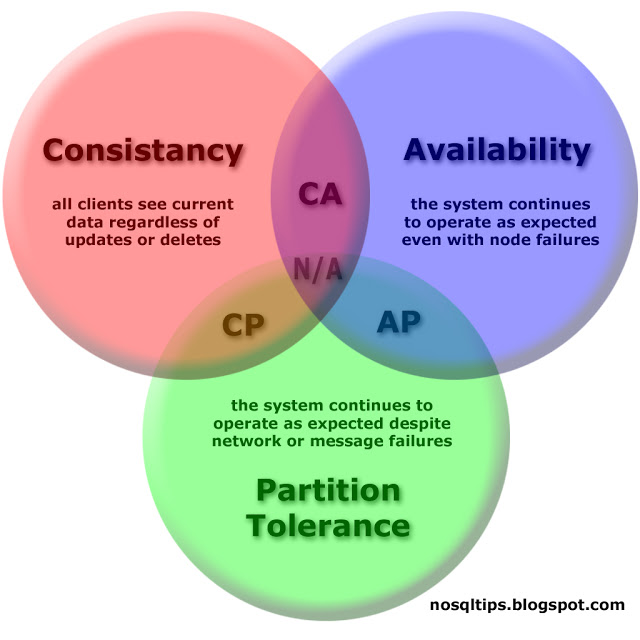
\includegraphics{figuras/CAP_Diagram}}
    \caption{Diagrama do Teorema de CAP(Brewer)}
    \label{submeter}
\end{figure}


\subsection{ C – Consistência }
É considerada como a característica que transcreve as duas condicionais de um sistema, como o sistema fica consistente após e
uma operação e se ele fica consistente. Uma base de dados consistênte distribuida é dita como fortemente consistente ou 
como tendo fraca consistência. Os sistemas com uma forte consistência, implementam as características ACID 
(Atomicidade, Consistência, Isolamento e Durabilidade), sendo estas implementadas na maior parte das bases de dados relacionais. 
Na outra extremidade, de fraca consistência, temos as bases de dados BASE (Basic Availability, Soft-State, Eventual 
Consistency).

\subsection{ A – Disponibilidade }
A disponibilidade que, segundo \cite{BROWNE}, deve garantir que um sistema esteja sempre fornecendo acesso e funcionalidades a seus usuários, 
é uma das propriedades mais importantes e indispensável para sistemas de empresas, sejam eles baseados em Web ou não mas  que precisam disponibilizar
seus serviços continuamente, por exemplo, empresas como a Google ou a Microsoft. Entretanto inevitáveis falhas podem ocorrer, e é nesse momento em que 
alguma contingência (backups automáticos e alguma redundância) deve ocorrer para minimizar o impacto ao usuário.

\subsection{ P – Tolerância ao Particionamento }
Tolerância ao particionamento significa assegurar que todas as operações sejam completadas, pode siginificar ao mesmo tempo a habilidade de um sistema
continuar operando, mesmo em situações em que componentes individuais já não estejam mais disponíveis, ou seja onde ocorra uma interrupção parcial de alguns 
componentes. "Assim, se um sistema disponibilizar essa propriedade, ele ainda será capaz de realizar operações como leitura e escrita mesmo após 
serem realizados diversos particionamentos na rede".\cite{GILBERT,NANCY}.

\section{NoSQL}
Muitas organizações que tradicionalmente coletam uma quantidade imensa de dados estruturados em bases de dados relacionais, em vista da demanda de dados incessantes crescendo
a todo momento, começaram a procurar novas soluções para armazenamento de dados acabando por optarem pelos bando de dados não relacionais, ou bando de dados não-SQL, que agora são 
frequentemente chamados de banco de dados NoSQL.

O termo NoSQL Database que pode ser entendido como \textbf{Not-Olny-SQL}, foi inicialmente anunciado em 1998, para bases de dados que omitiam a linguagem SQL, um termo genérico re-introduzido por \cite{EVANS} da Rackspace,
durante um movimento chamado \textbf{\textit{ NoSQL meetup in San Francisco}}, promovido Johan Oskarsson da \textbf{ Last.fm } um site com objetivo de criar uma rádio online agregando uma comunidade virtual com foco em música; o evento foi criado com o intuito de descrever 
bases de dados que não mais se dispõem do uso de SQL tais como:\textbf{ Mysql, PostgreSQL, Oracle, SQLServer }(...) em suas transações, sejam elas de manipulação ou consulta de dados. O principal foco era discutir o crescimento e surgimento de novas 
além de apresentar soluções ou novas alternativas open-source de armazenamento de dados distribuidos não relacionais. Os NoSQL surgiram como uma solução para a questão de escalonamento, concistência e disponibilidade no
armazenamento e processamento de grandes volumes de dados na \textbf{WEB 2.0}.

"Ao que tudo indica o termo noSQL foi criado em 1998 por Carlo Strozzi para nomear seu projeto open source, que tinha como objetivo ser uma implementação mais leve de um banco de dados relacional, 
porém sua principal característica era não expor a interface SQL."\cite{DEVMEDIA}

A principal característica dos noSQL é o fato de não apresentarem a linguagem SQL, e essa iniciativa de retirar as estruturas impostas pelos SGBDs baseados no modelo relacional de dados, garante que os noSQL em determinadas ocasiões, busquem: acelerar, otimizar e organizar os dados de 
maneira de objetiva direta e livre de relacionamentos, todavia a diferença mais importante e incessantemente discutida entre as base de dados não relacionais é a da alta escalabilidade necessaria para gerenciar enormes volumes de dados, tornando estes mais flexiveis as caracteristicas 
\textbf{ACID}, onde os atuais banco de dados relacionais são muito restritos quanto a escalabilidade pois fazem uso de escalonamento vertical ou seja quanto mais dados trafegarem mais espaço é solicitado e com isso mais memória é necessario para manter o servidor conciso na maipulação 
do volume de dados. A diferença única e exclusivamente se encontra no escalonamento, os noSQL fazem uso do escalonamento horizontal e possuiem maior facilidade de distribuição de dados, ou seja com o aumento do numero de dados, surge-se a necessidade de aumentar o numero de servidores, 
otimizando o desempenho e performance do armazenamento.

\subsection{ Escalonamento horizontal }
Como fora mencionado na sessão acima sobre escalonamento horizontal, este tende a ser uma solução mais confiável, apesar de possuir alguns requerimentos como diversas threads/processos distribuidos, ou seja fazendo uma divisão desses dados em varios outros servidores distribuidos, minimizando o volume de dados por servidor, 
e neste caso menos processamento e gerenciamento de dados e memória são gastos, tornando determinada situação mais simplificada. Neste caso o uso de uma base de dados relacional começa a se tornar inviável, uma vez que com um número de processos distribuidos conectados simultaneamente à um mesmo modelo de dados relacional, 
causaria uma alta concorrência entre os mesmos, fazendo com que haja um tempo maior de acesso às tabelas envolvidas bem como seus relacionamentos. 

"Quando pensamos na arquitetura de sistemas com grande volume de dados a primeira palavra que vem a mente é escalar. Além de desejar que cada uma das pesquisas em nosso sistema execute o mais rápido possível, precisamos criar meios para que, quando necessário, seja fácil adicionar mais recursos (como memória ou novos servidores) e o sistema consiga tirar proveito deles. Para isso muitas vezes precisamos ir além das diversas otimizações de performance e escalabilidade, como por exemplo a criação de um índice para buscas, o uso de caches e de chamadas assíncronas." \cite{ALMEIDA,SILVEIRA}

Para que seja permitido o escalonamento horizontal, deve existir a ausência de bloqueio, o que torna essa tecnologia mais adequada e capaz de solucionar problemas quanto ao gerenciamento do grande volume de dados que crescem exponencialmente, assim como os dados na WEB 2.0. Existem duas abordagens \textit{\textbf{replicação e particionamento horizontal}} de extrema importância para se conseguir o escalonamento horizontal. Replicação possui uma idéa bastante diversificada por muitos, porem
 neste caso siguinifica, dividir toda e qualquer parte da base de dados em multiplas partes e as armazenando em mais de um nó na rede. A implementação desta técnica pode muito bem ser criada através de uma clássica estrutura vista em diversos outros sistemas distribuidos
a estrutura \textbf{master-slave} de processos se comunicando através de troca de mensagens. 

Segundo \cite{SLOMAN}, "Um sistema de processamento distribuído é tal que, vários  processadores e dispositivos de  armazenamento de dados,  comportando processos e/ou bases de  dados, interagem cooperativamente  para alcançar um objetivo comum. Os  processos coordenam suas atividades e  trocam informações por passagem de  mensagens através de uma rede de comunicação".

A aplicação da técnica de escalonamento horizontal, também conhecida como \textbf{Sharding}, faz com que as queries possam ser executadas em mais de um nó e quando da sobre-carga dos servidores um novo nó escravo(slave), é criado aliviando os trabalhos ocorridos nos demais nós encontrados na base de dados. Uma vantagem dessa técnica está em caso um desses nó pare ou aconteça algum
conflito, não haverá segundo pesquisadores, problemas com as queries, uma vez que outros nós podem responder pelos mesmos processos.





\subsection{ NoSQL 1: Sistemas CP }

\subsection{ NoSQL 2: Sistemas AP }

\section{Comparativo entre SGBDS Relacionais e Não Relacionais}
